\chapter{Aplikace}
Vzhledem ke komplexnosti aplikace je pro přehlednost rozdělena do několika složek. Podobným způsobem byly rozděleny Class diagramy projektu, 
\section{Prisma}
\label{sec:prisma}
Databázové schéma v jazyku Prisma a databázové migrace se nachází ve složce \code{/prisma/}. Po úpravě databázové schématu je vhodné i vytvořit databázovou migraci, ta umožní manuálně spustit SQL příkazy, které Prisma vykonala, pokud to bude potřeba. Díky použití Prismy lze jak na API tak na frontendové části aplikace používat identické datové typy, nemusíme, především na Frontendu, definovat vlastní "Interface" pro každý objekt v databázi, který bychom museli pokaždé aktualizovat, když se změní databázové schéma, databázové schéma tedy může fungovat i jako Class diagram.
Následuje vizualizace databázové schématu vygenerovaná pomocí webové aplikace Prismaliser \cite{prismaliser}.

\begin{landscape}
\begin{figure}[hbt]
	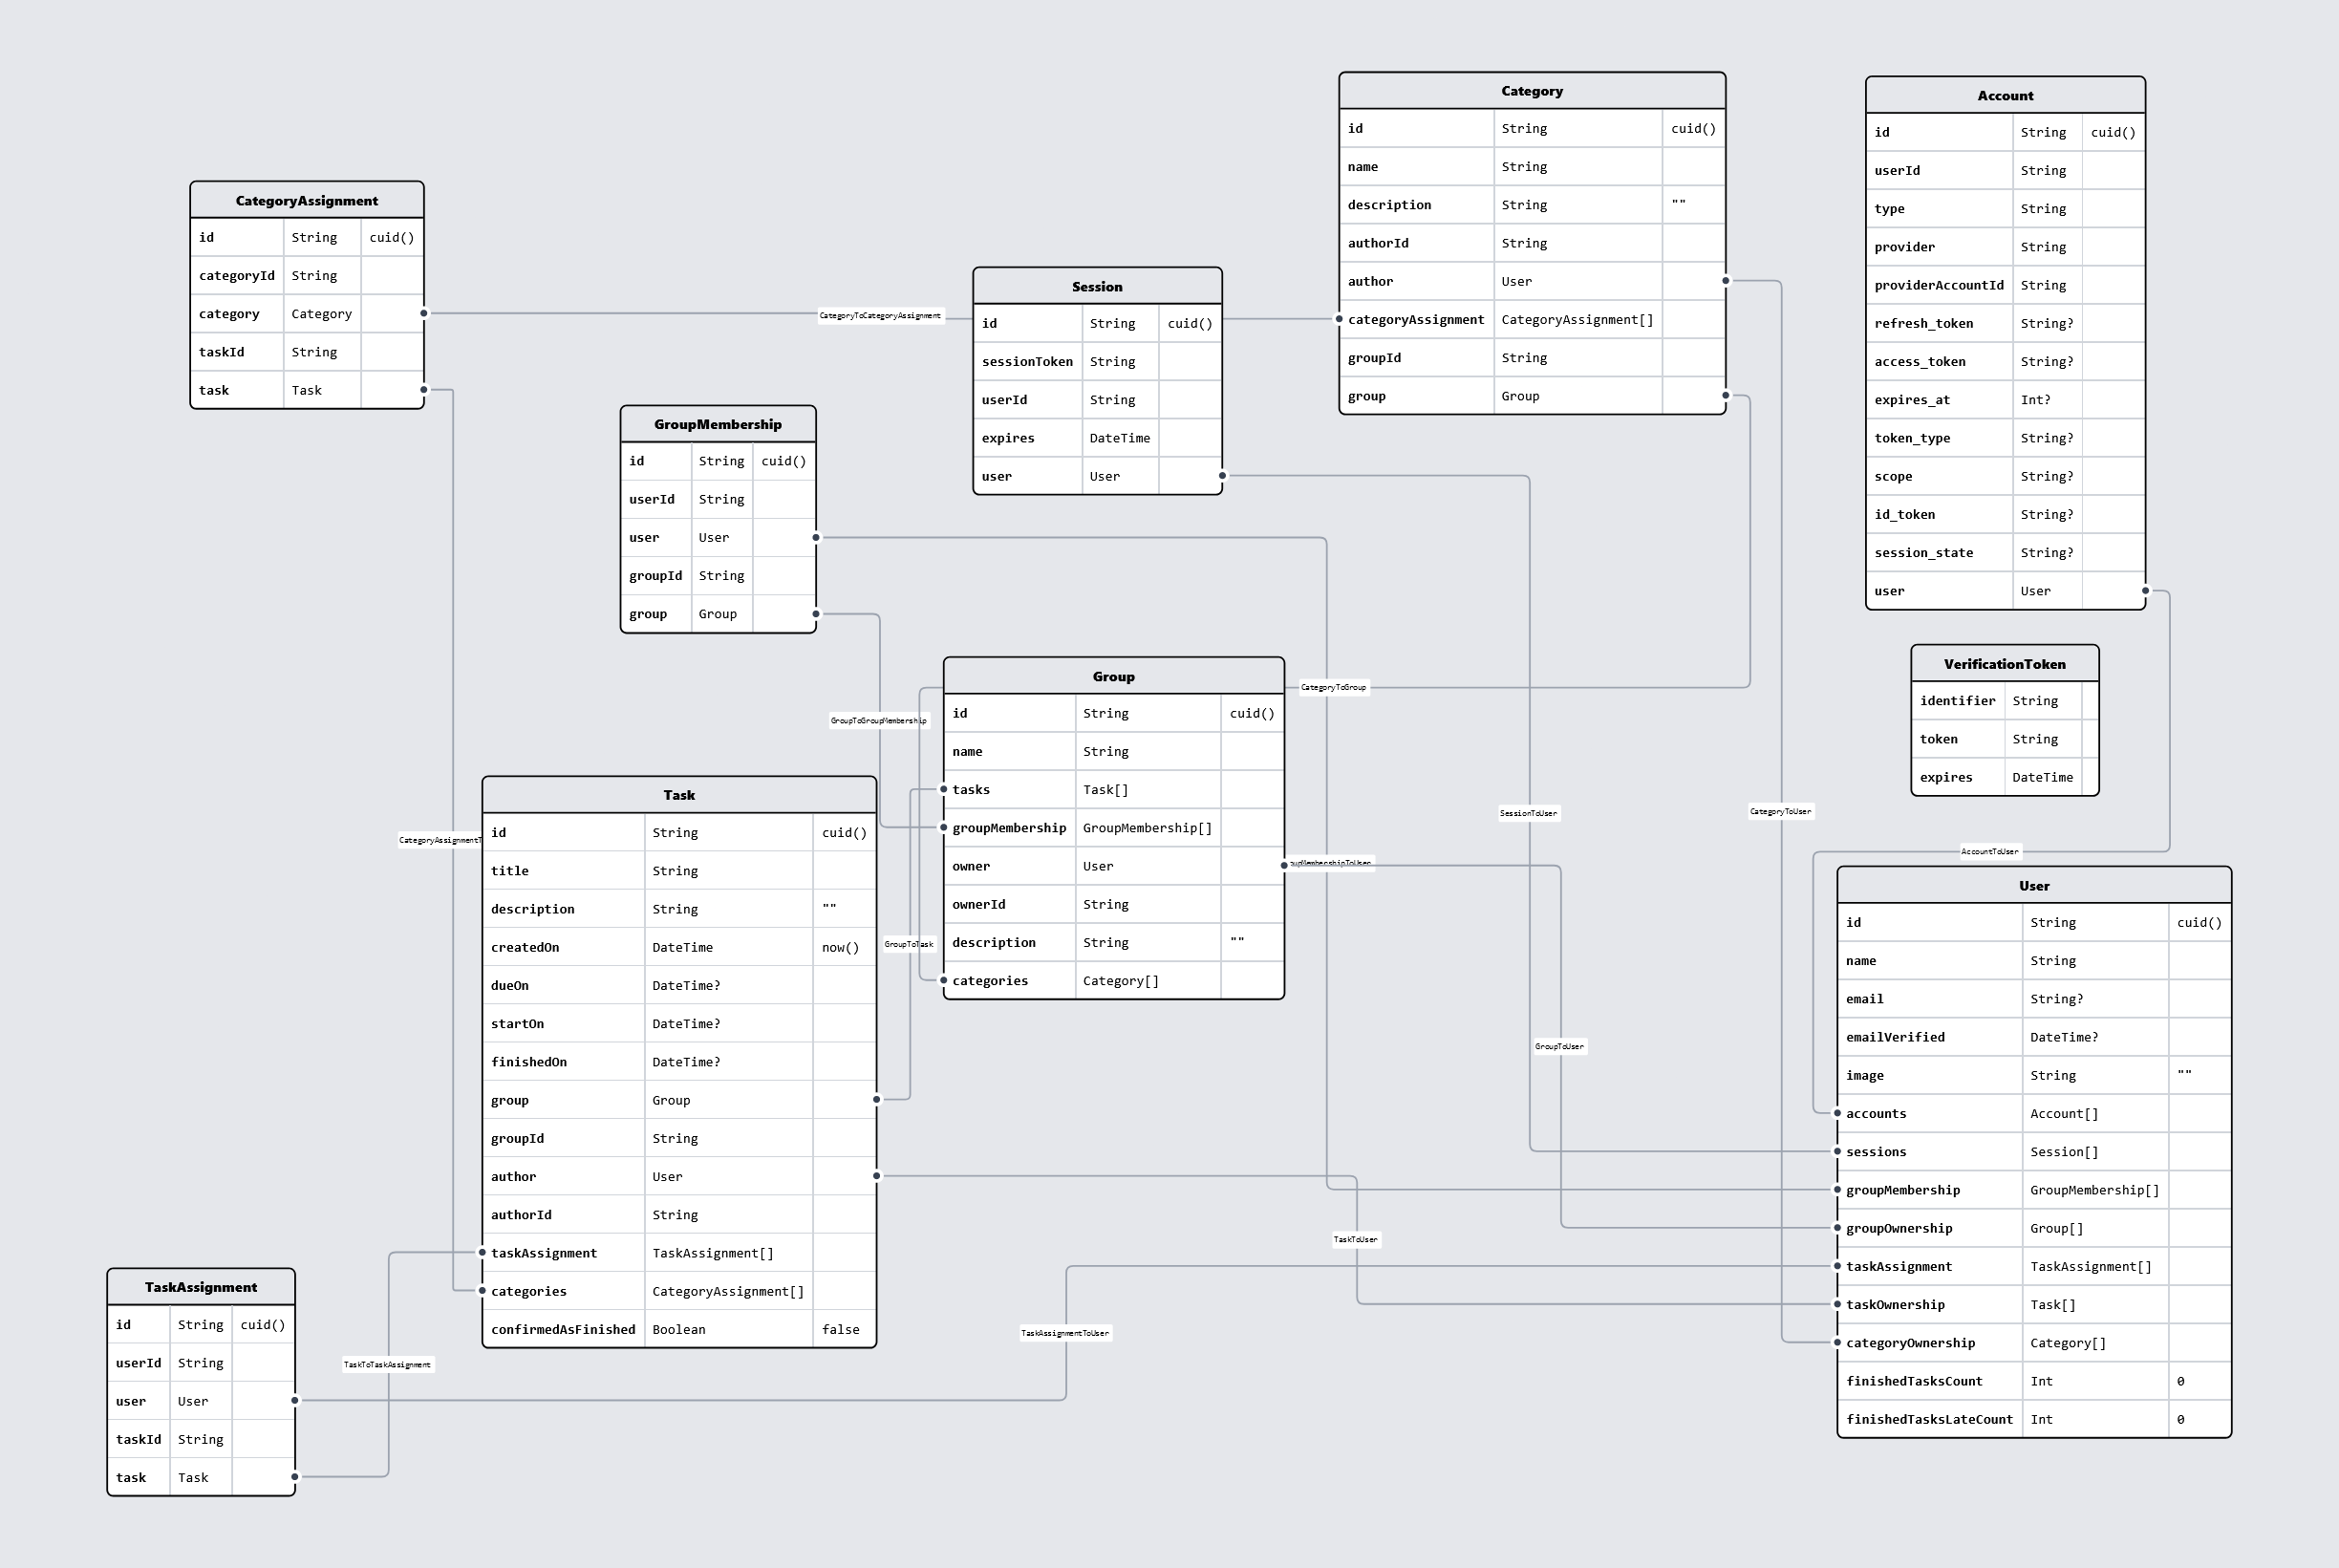
\includegraphics[width=1\linewidth]{img/DB_schema.png}
	\caption{Databázové schéma}
\end{figure}
\end{landscape}
\section{API}
\label{sec:api}

Celé API je psané za pomocí tRPC, to se nachází ve složce \code{/src/server/api/}.
API je inicializováno v souborech \code{trpc.ts} a \code{root.ts}. Konktrétně v souboru \code{trpc.ts} inicializujeme objekt tRPC a v \code{root.ts} se na něj napojují jednotlivé Routery. Samotné "endpointy", tedy přístupy, jsou rozděleny do "routerů", ty se nachází ve složce \code{/src/server/api/routers} a dělí se na jednotlivé "hlavní objekty" v databázi. Tyto routery jsou děleny na soubory \code{categories.ts}, \code{groups.ts}, \code{tasks.ts} a \code{users.ts}. V kódu se "endpointy" označují jako "procedury", v princpu existují dva druhy procedur; public\footnote{Veřejná} a protected\footnote{Chráněná}. Jediným rozdílem mezi nimi je, že protected procedura zaručuje, že jí může úspěšně zavolat pouze přihlášený uživatel.
Následuje úryvek z routeru pro skupiny v souboru \code{groups.ts}, ostatní procedury byly z ukázky odstraněny.
\begin{lstlisting}[caption={Procedura na přidání uživatele do skupiny}]
import { z } from "zod";

import {
  createTRPCRouter,
  protectedProcedure,
  publicProcedure,
} from "~/server/api/trpc";

export const groupsRouter = createTRPCRouter({
...
addMember: protectedProcedure
    .input(z.object({ userId: z.string(), groupId: z.string() }))
    .mutation(async ({ ctx, input }) => {
      const group = await ctx.prisma.group.findFirst({
        where: { id: input.groupId },
      });
      if (!group)
        throw new TRPCError({ code: "NOT_FOUND", message: "Group not found" });
      const user = await ctx.prisma.user.findFirst({
        where: { id: input.userId },
      });
      if (!user)
        throw new TRPCError({ code: "NOT_FOUND", message: "User not found" });
      if (group.ownerId !== ctx.session.user.id)
        throw new TRPCError({
          code: "UNAUTHORIZED",
          message: "Must be owner of the group",
        });
      const membership = await ctx.prisma.groupMembership.create({
        data: {
          groupId: input.groupId,
          userId: input.userId,
        },
      });
      if (membership) return true;
      return false;
    }),
})
\end{lstlisting}
Jako první je nutné definovat název Procedury, v tomto případě "addMember", tedy "přidatUživatele". Dále přidáme \code{.input()} zde bude procedura přijímat data pro své provedení. Pokud bude Procedura data měnit tak přidáme \code{.mutation}, pokud data pouze předá z databáze, tak přidáme \code{.query}. Do nich poté předáme vstup z \code{.input} a \code{ctx}\footnote{Kontext}. Kontext je globálně zpracovávaný a nachází se v něm \code{session} přihlášeného uživatele a \code{prisma}, tou se napojujeme na databázi.
\newpage
\subsection{Příklad API Endpointů}

Následující tabulka zobrazuje vybrané API Endpointy, z každého routeru, který se v aplikaci nachází dva Endpointy. Tyto Endpointy byly vybrány vzhledem k jejich četnosti výskytu v aplikaci, ale také vzhledem k jejich rozmanitosti přijímaných a vracených dat.
\begin{table}[hbt!]
    \centering
    \begin{tabularx}{1\textwidth} { 
	| >{\centering\arraybackslash}X 
	| >{\centering\arraybackslash}X 
	| >{\centering\arraybackslash}X 
	| >{\centering\arraybackslash}X 
	| >{\centering\arraybackslash}X | }
	\hline
	\textbf{Router} & \textbf{Název} & \textbf{Popis}                                                  & \textbf{Vstup}                       & \textbf{Výstup} \\
	\hline
	categories.ts   & create          & Vytvoří kategorii                                             & Název, Popis, ID autora, ID skupiny & Category         \\
	\hline
	categories.ts   & getTasks        & Vrátí úkoly s kategorií                                     & ID kategorie                         & Task[]           \\
	\hline
	tasks.ts        & assignUser      & Přiřadí uživatele k úkolu                                  & ID uživatele, ID úkolu             & True / False     \\
	\hline
	tasks.ts        & getCategories   & Vrátí pole kategorií úkolu                                  & ID úkolu                            & Category[]       \\
	\hline
	groups.ts       & getById         & Vrátí objekt skupiny, pokud je přihlášený uživatel člen & ID skupiny                           & Group            \\
	\hline
	groups.ts       & leave           & Odstraní přihlášeného uživatele ze skupiny                & ID skupiny                           & True / False     \\
	\hline
	users.ts        & locateByName    & Vrátí pole uživatelů s podobným jménem k vstupu           & Text                                 & User[]           \\
	\hline
	users.ts        & editName        & Upraví jméno uživatele                                       & ID uživatele, Nové jméno          & User             \\
	\hline
\end{tabularx}
    \caption{Příklad API Endpointů}
    \label{tab:my_label}
\end{table}

\newpage
\section{Next.js}
Kód, ze kterého se staví frontendová část aplikace pomocí Next.js se nachází ve složkách \code{src/pages} a \code{src/components}. V \code{pages} se nachází webové stránky, které vidí uživatel, v \code{components} jsou uloženy komponenty, ze kterých se staví jednotlivé stránky.
Obě složky jsou rozděleny do podsložek podle jednotlivých objektů, kterých se týkají, například v \code{src/components/groups} se nachází pouze komponenty, které se týkají skupin.
\subsection{src/components/}
Složka je rozdělena na následujících podsložek:
\dirtree{%
	.1 components.
	.2 auth //komponenty související s autorizací uživatelů. 
	.2 categories //komponenty související s kategoriemi.
	.2 groups //komponenty související se skupinami.
	.2 layout //komponenty související s rozvržením stránek.
	.2 tasks //komponenty související s úkoly.
	.2 users //komponenty související s uživateli.
}
\hfill \break
Jednotlivé podsložky jsou následně rozděleny na komponenty, které mají každá svou vlastní složku.
Ve složce pro komponentu se nachází soubor \code{index.tsx} a \code{názevKomponenty.tsx}.
\hfill \break
Finálně tedy struktura adresáře vypadá následovně:
\dirtree{%
	.1 /.
	.2 src.
	.3 components.
	.4 příbuznéKomponenty.
	.5 názevKomponenty.
	.6 index.tsx.
	.6 názevKomponenty.tsx.
	.3 pages.
}
Jednotlivé komponenty jsou vnořeny ve vlastních složkách, aby bylo možné je odděleně stylovat, pokud to bude nutné, pomocí css, nebo scss, tohoto se využívá v komponentě \code{taskCalendar}.
\subsubsection{Proč přidat do složky i index.tsx}
Abychom mohli komponentu na stránce použít musíme ji importovat pomocí příkazu \code{import}, pro ukázku jsem se rozhodl použít komponentu \code{pageHeader}
\begin{lstlisting}
    import PageHeader from "~/components/layout/pageHeader/pageHeader";
\end{lstlisting}
Zde je patrné, že v příkazu máme zdvojeně název komponenty, protože máme komponenty rozdělené do jednotlivých složek a poté je máme pojmenované jménem. Jedním z řešení, jak dosáhnout \code{import}u, co vypadá následovně je přejmenovat komponenty z názvu na \code{index.tsx}.
\begin{lstlisting}
    import PageHeader from "~/components/layout/pageHeader/";
\end{lstlisting}
Adresář by tedy vypadal následovně:
\dirtree{%
	.1 /.
	.2 src.
	.3 components.
	.4 příbuznéKomponenty.
	.5 názevKomponenty.
	.6 index.tsx.
	.3 pages.
}

Pokud bychom přejmenovali komponenty na \code{index.tsx} tak sice dosáhneme požadovaného výsledku, ale pokud bychom ve vývojovém prostředí měli otevřeno několik komponent, byl by problém se v projektu zorientovat.
Proto místo přejmenování komponent na \code{index.tsx} ponecháme soubor pojmenovaný názvem komponent a vytvoříme pro každou komponentu jejich vlastní soubor \code{index.tsx}, tímto způsobem docílíme nezdvojené adresy v \code{import}u, protože když \code{import} dostane jako cestu složku automaticky vybere soubor s názvem \code{index.tsx}. Následně v souboru \code{index.tsx} musíme importovat komponentu, které se týká a tu dále exportovat. Složka komponenty a její soubory vypadají následovně, irelevantní části kódu byly vynechány.
\begin{lstlisting}[caption=Deklarace komponenty pageHeader]
...
const PageHeader: React.FC<Props> = (props: Props) => {
  return (
    ...
  );
};

export default PageHeader;
\end{lstlisting}
\begin{lstlisting}[caption=Soubor index.tsx komponenty pageHeader]
import PageHeader from "./pageHeader";
export default PageHeader;
\end{lstlisting}
\subsection{/src/pages/}
Struktura adresáře \code{pages} vypadá následovně:
\dirtree{%
	.1 pages.
	.2 api.
	.2 groups.
	.2 tasks.
	.2 users.
	.2 \_app.tsx.
	.2 404.tsx.
	.2 500.tsx.
	.2 index.tsx.
}
\hfill \break
Ve složce \code{api} se nachází soubory pro inicializaci API a NextAuth na Frontendu, dále se zde nachází stránka \code{panel.ts}. K té je povolen přístup pouze ve vývojovém prostředí, jinak vždy vrací kód 404. Stránka byla použita během vývoje na testování API. NextAuth je incializován v souboru \code{/auth/[...nextauth].ts} a tRPC je inicalizováno v \code{/trpc/[trpc].ts}.

\subsubsection{\_app.tsx}
Soubor \code{\_app.tsx} je stavební kámen celé uživatelské části aplikace, tato stránka funguje, jako šablona pro všechny stránky aplikace. Na stránce pomocí komponenty \code{checkAuth} aplikace kontroluje na všech stránkách, kromě stránky index, zda je uživatel přihlášen a pokud ne, zobrazí uživateli pouze žádost o to, aby se přihlásil.

\begin{lstlisting}[caption=Komponenta CheckAuth]
...
type Props = {
  children: ReactNode;
};

const CheckAuth: FC<Props> = ({ children }) => {
  const router = useRouter();
  const isIndexPage = router.pathname === "/";
  const { status } = useSession();
  if (isIndexPage) return <>{children}</>;
  if (status === "loading") return <Loading />;
  if (status === "unauthenticated") return <SignIn />;
  if (status === "authenticated") return <>{children}</>;
  return <Code500 />;
};

export default CheckAuth;

\end{lstlisting}
CheckAuth přijímá jako parametr \code{children}, tedy děti, ty komponentě nepředáme stejným způsobem jako ostatní parametry, ale vložením dětí mezi otevírací a uzavírací značky.
\begin{lstlisting}[caption=Standardní předání parametrů komponentě]
    <PageHeader name="Calendar" breadcrumbs={[]} />
\end{lstlisting}
\begin{lstlisting}[caption=Předání dětí komponentě]
    <CheckAuth>
        <Component {...pageProps} />
    </CheckAuth>
\end{lstlisting}
\section{Rozvržení uživatelských práv}
Uživatelé se nacházejí, po přidání vlastníkem, ve skupinách, skupiny mají pod sebou úkoly a kategorie. Aby byl uživateli vylepšen prvotní zážitek při používání aplikace, tak mu je automaticky s účtem i vytvořena skupina. Samozřejmě si uživatelé mohou v aplikaci spravovat nové skupiny. Ve skupinách poté mohou vytvářet úkoly a kategorie, kategorie mohou být přiřazeny jednotlivým úkolům. Majitelé skupin mohou upravovat členství uživatelů ve skupině, vlastnosti skupiny, jako například název nebo převést skupinu na dalšího uživatele. 

U úkolů a kategorií mohou úpravy provázet jen autoři a také majitel skupiny pod kterou spadají. Po odebrání, nebo odchodu uživatele ze skupiny, se veškeré úkoly převedou na majitele skupiny. 
\newpage
\subsection{Diagramy}
Pro přehlednost byl UseCase diagram rozdělen na dvě části, UseCase diagram aplikace a UseCase diagram v zobrazení skupiny.

\begin{figure}[hbt!]
	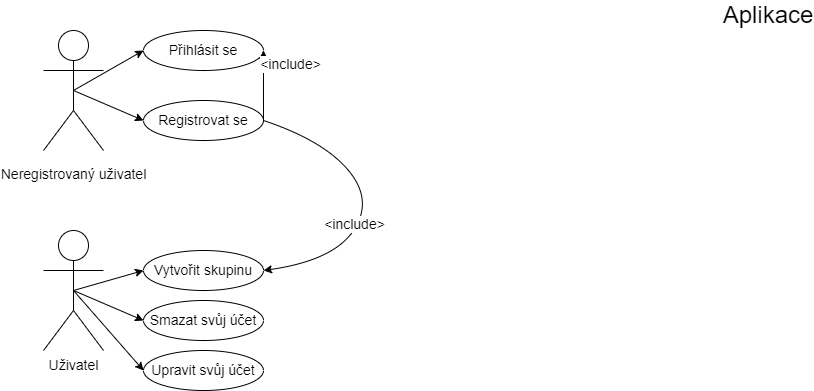
\includegraphics[width=0.8\linewidth]{img/UseCaseAplikace.png}
	\caption{UseCase Diagram aplikace}
\end{figure}

Následující UseCase diagram zobrazuje akce, které mohou uživatelé provádět ve skupině.
\begin{figure}[hbt!]
	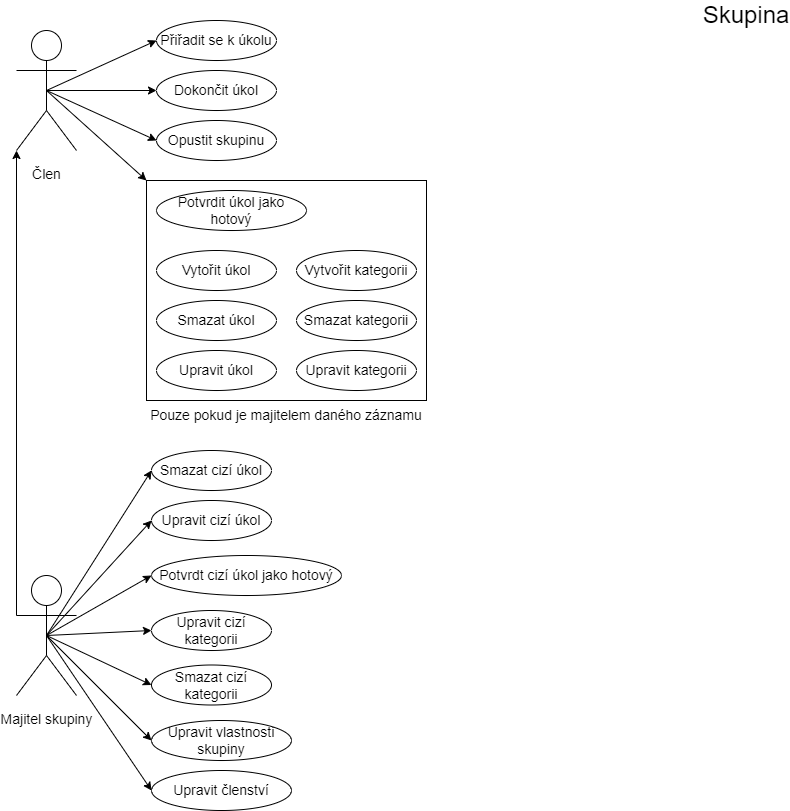
\includegraphics[height=0.7\textwidth]{img/UseCaseSkupina.png}
	\caption{UseCase Diagram skupiny}
\end{figure}
\clearpage
\section{Uživatelské rozhraní}
Uživatelské rozhraní aplikace je poměrně jednoduché v horní části aplikace se nachází navigační panel. V navigačním panelu se nachází název aplikace, odkaz na úkoly, kalendář a skupiny přihlášeného uživatele. Pokud uživatel není přihlášen tak se v navigačním panelu nachází i tlačítko pro přihlášení, jakmile se uživatel přihlásí tak tlačítko zmizí a je nahrazeno jeho profilovým obrázkem, ten slouží jako odkaz na stránku uživatele. 

Výchozí nastavení, které používá T3 Stack je uložit odkaz na profilový obrázek z účtu, pomocí kterého se přihlásil uživatel do aplikace. Toto řešení je poměrně "nešťastné", protože při každém vstupu do aplikace se musí provést volání na externí službu, kde aplikace uživatelův obrázek stáhne. Z tohoto důvodu jsem se rozhodl použít pro generování profilových obrázků knihovnu \code{DiceBear}\cite{dicebear}. Tato knihovna poskytuje rozhraní pro vytváření různých avatarů formátu SVG.

\subsection{Registrace do aplikace}
Jakmile NextAuth zachytí událost typu registrace nového uživatele, tak zavolá tuto knihovnu a ta mu vytvoří nový profilový obrázek, ten je následně převeden na text a uložen do databáze. Jako "seed" pro generaci je použito uživatelovo \code{ID} a jako skupinu avatarů aplikace používá "lorelei-neutral"\cite{lorelei-neutral}. Při odchytnutí nového uživatele je také pro tohoto uživatele automaticky vytvořena nová skupina.

Jakmile je na serveru zachycena událost\footnote{Tedy "Event"} o vytvoření nového uživatele, NextAuth tento Event vyvolá pokaždé co se zaregistruje nový uživatel do aplikace vytvoří se nový záznam v databázi. Při vytvoření uživatele je vygenerován nový uživatelský obrázek pomocí knihovny DiceBear. Po vygenerování obrázku je obrázek převeden na \code{DataURI} a uložen do databáze. Po uložení obrázku je uživatelovi dále vytvořena první skupina, ta je vytvořena pro ulehčení a zjednodušení prvního vstupu do aplikace.

\begin{figure}[hbt!]
	
\includegraphics[width=1\linewidth]{img/neprihlasenyNavbar.png}
	\caption{Navigační panel nepřihlášeného uživatele}
\end{figure}
\begin{figure}[hbt!]
	
\includegraphics[width=1\linewidth]{img/prihlasenyNavbar.png}
	\caption{Navigační panel přihlášeného uživatele}
\end{figure}
\clearpage
Na každé stránce, která není úvodní, je nepřihlášený uživatel požádán o přihlášení a není vpuštěn do aplikace.

\begin{figure}[hbt!]
	\centering
	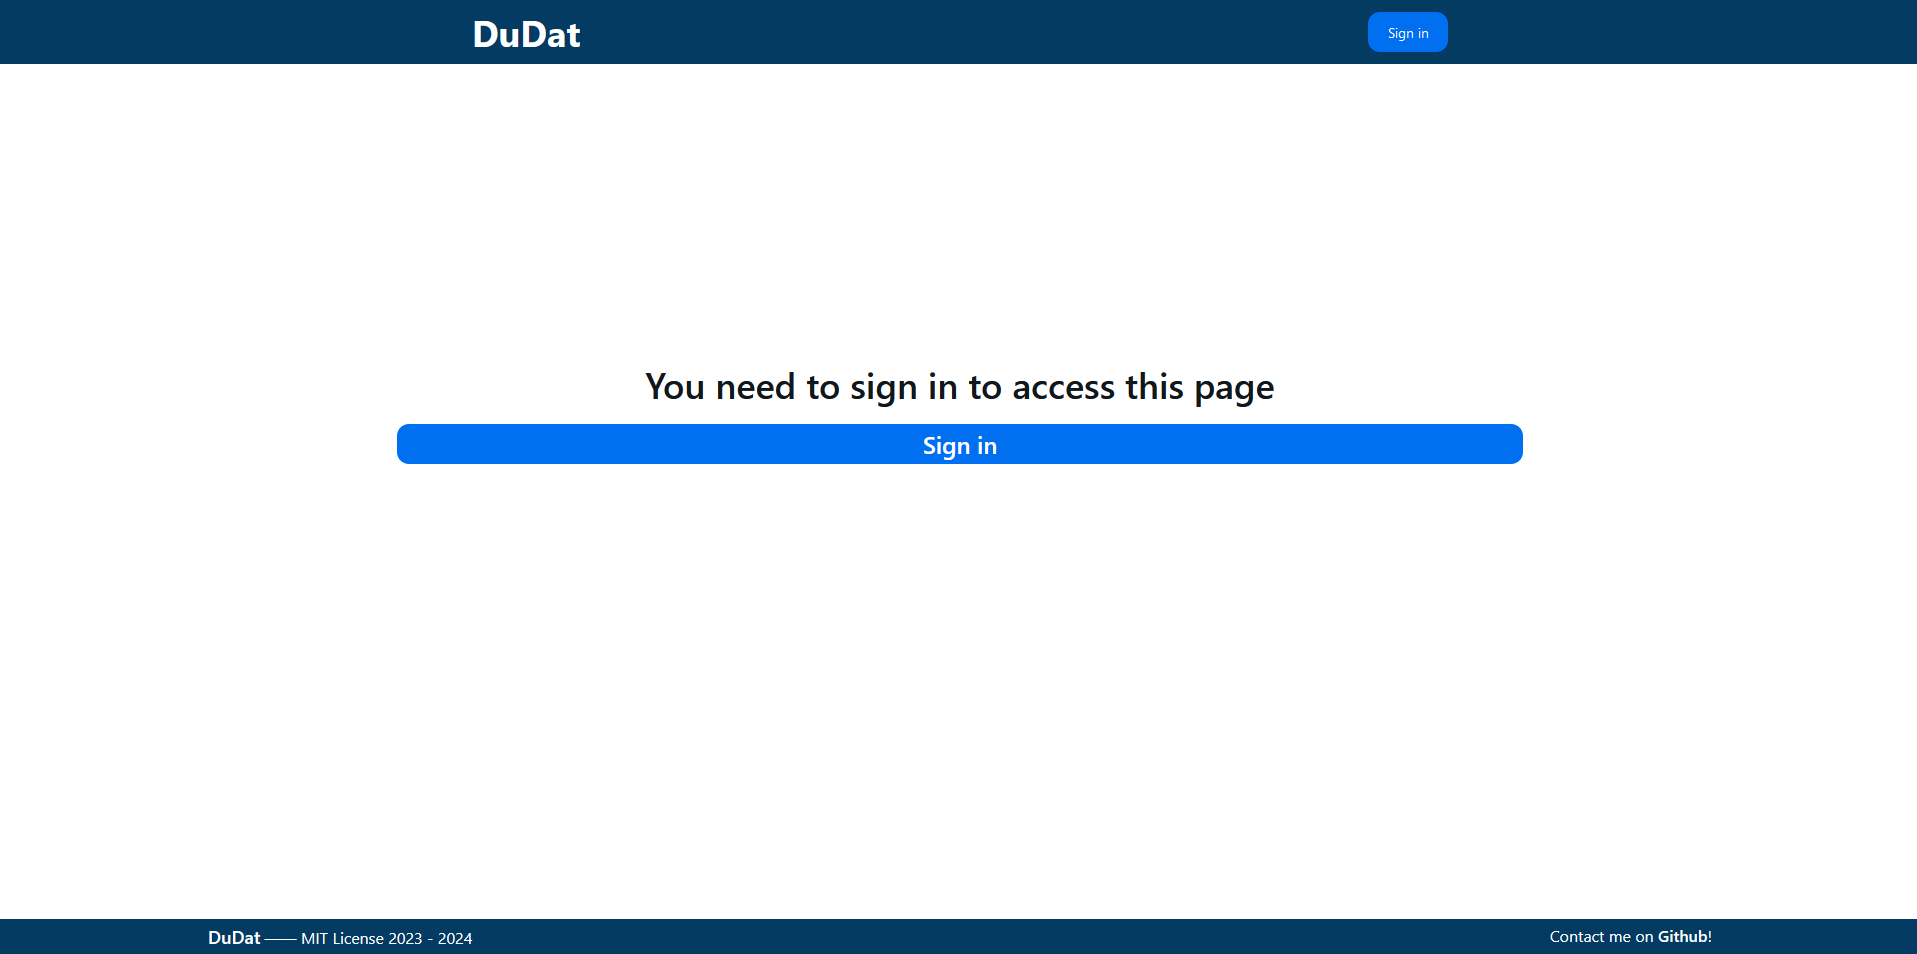
\includegraphics[width=1\linewidth]{img/signIn.png}
	\caption{Stránka se žádostí o přihlášení}
\end{figure}
Na stránku skupiny, úkolu a kategorie se dostanou pouze členové dané skupiny, vlastníkovi se místo tlačítka pro opuštění skupiny zobrazí tlačítko pro vstup do nastavení skupiny.
\begin{figure}[hbt!]
	\centering
	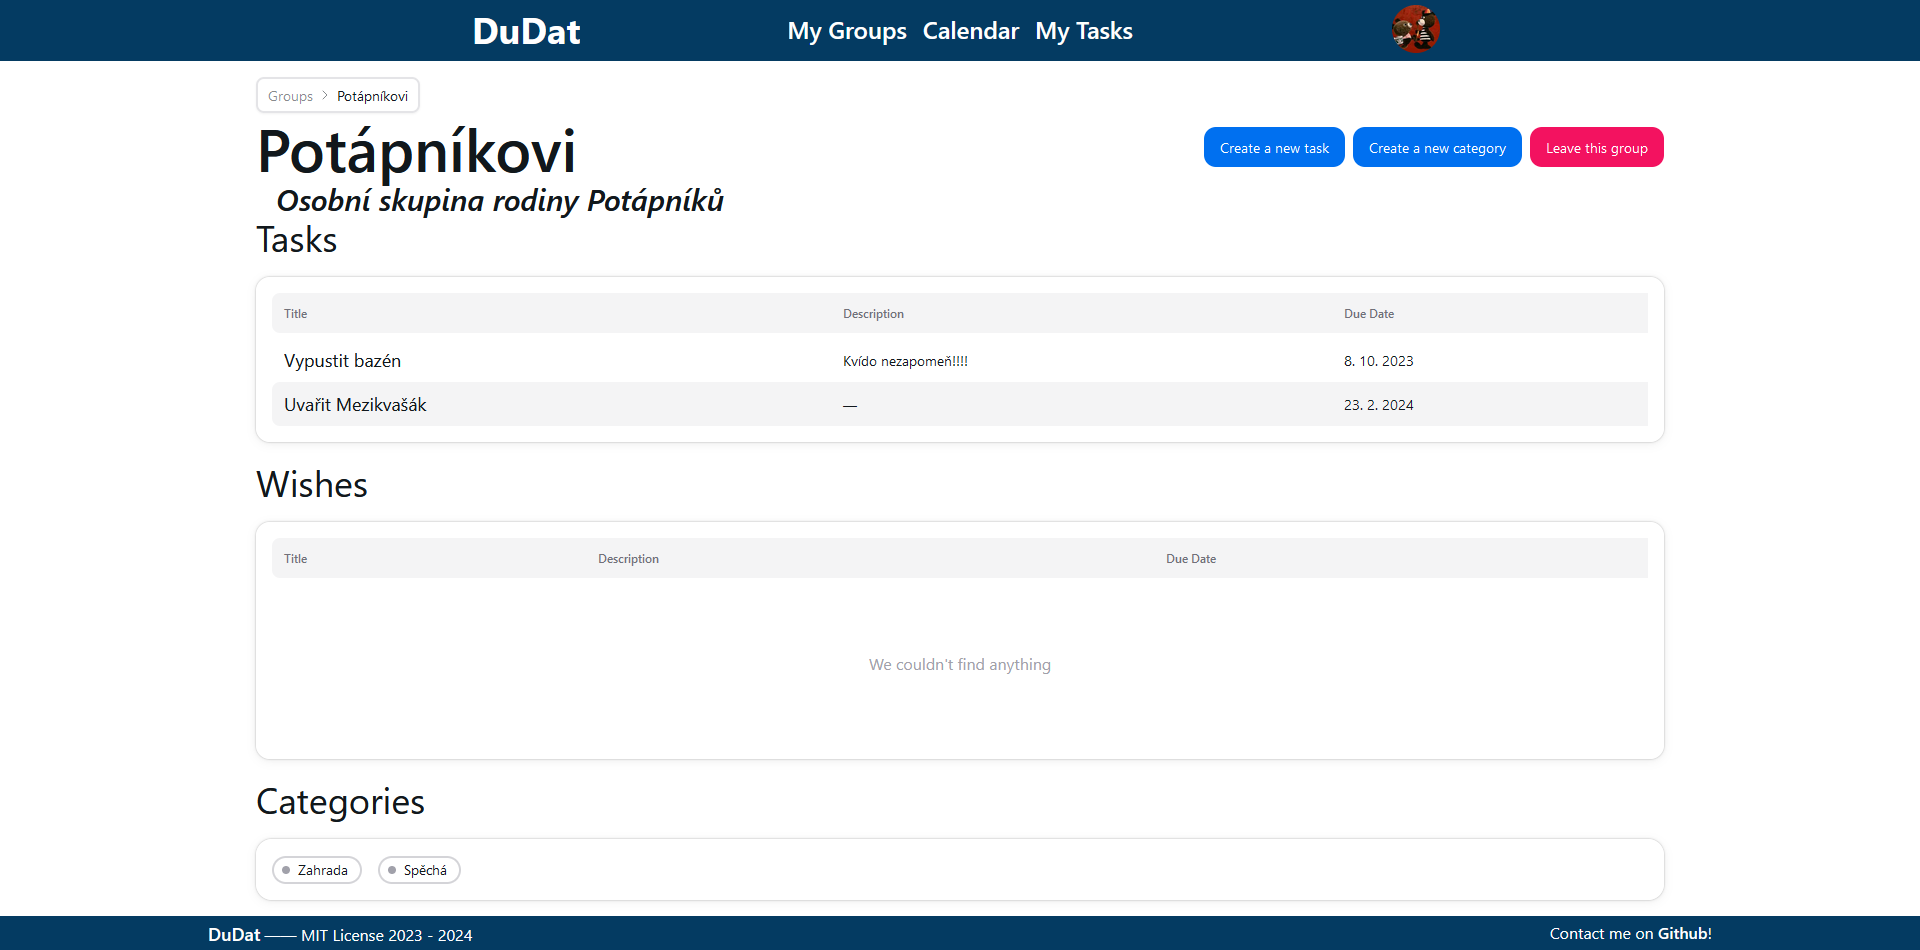
\includegraphics[width=1\linewidth]{img/groupPage.png}
	\caption{Zobrazení skupiny z pohledu člena}
\end{figure}
Na stránkách skupiny vidíme výpis úkolů, přání, kategorií a ostatních členů v dané skupině. Na stránkách úkolu vidíme přiřazené uživatele, možnost se "odhlásit" nebo "přihlásit" k plnění úkolu, tlačítko pro dokončení úkolu, kategorie a indikátor do kdy má být daný úkol hotov. Autor úkolu a majitel skupiny dále vidí panel pro nastavení, kde může úkol upravit a potvrdit ho jako vypracovaný.

\begin{figure}[hbt!]
	\centering
	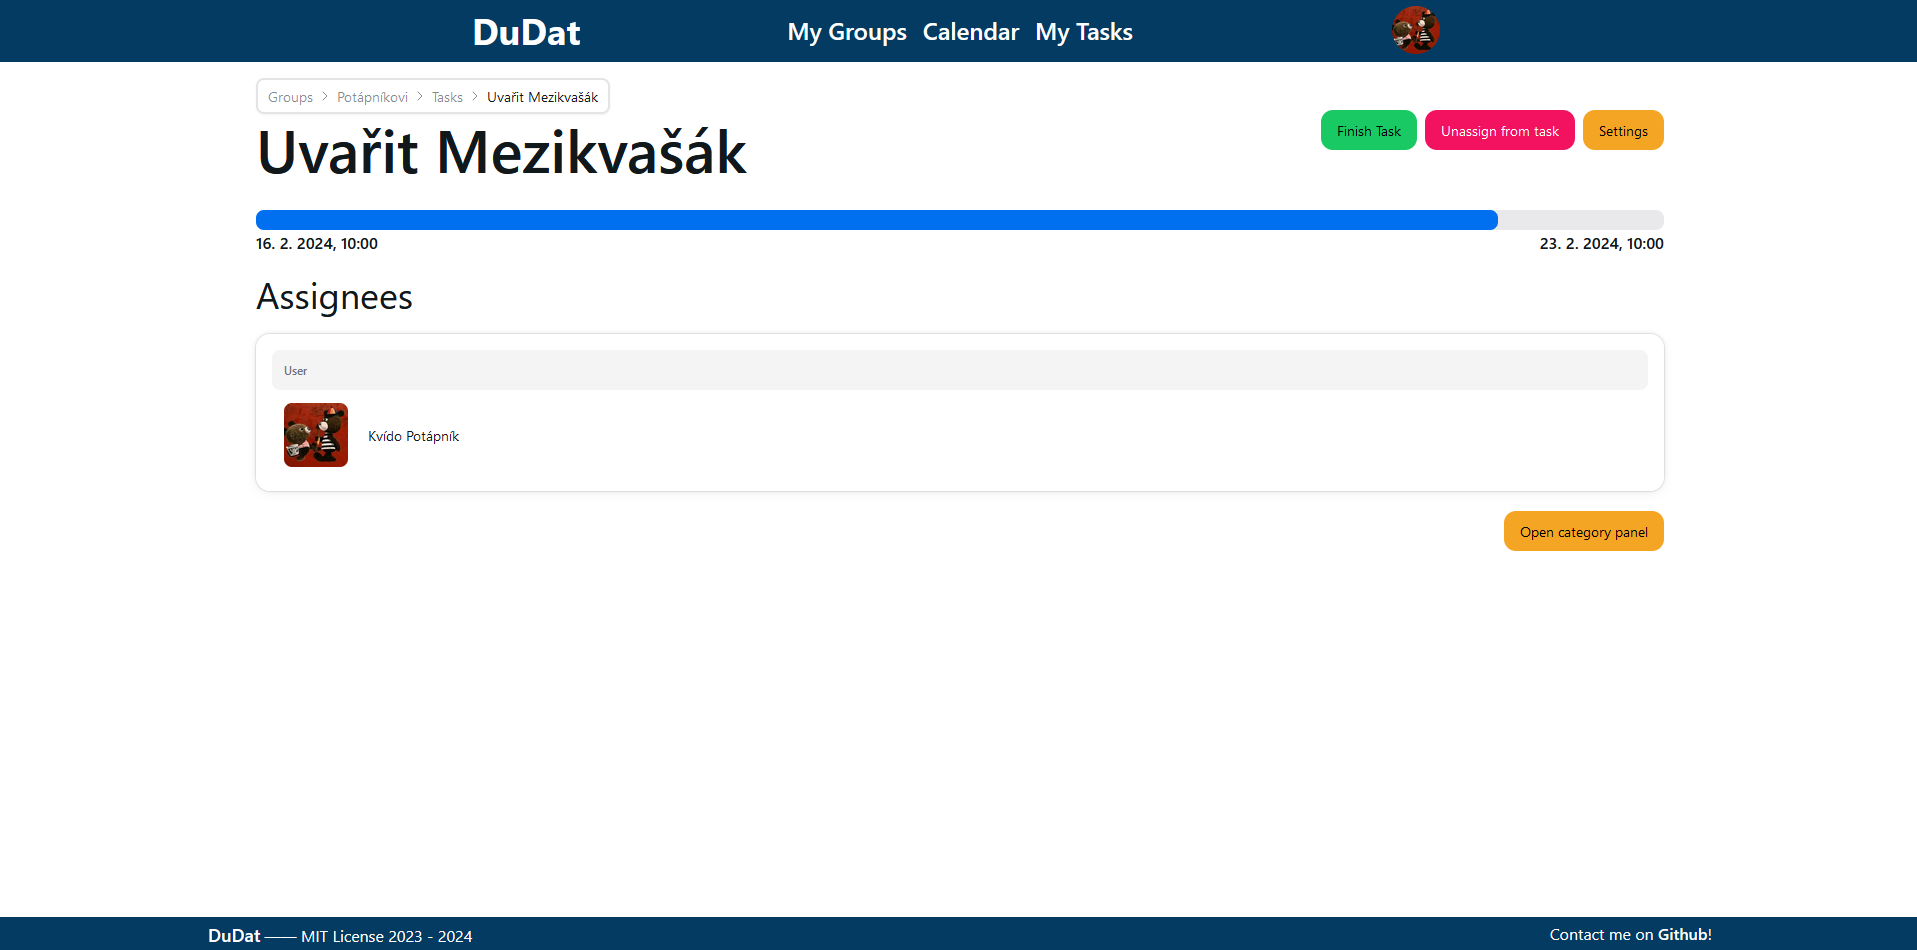
\includegraphics[width=1\linewidth]{img/ukol.png}
	\caption{Zobrazení úkolu z pohledu majitele\cite{mezikvasak}}
\end{figure}


Když je na vypracování úkolu stále čas, tak je indikátor modrý, jakmile se blíží konec lhůty na vypracování, konkrétně když zbývá méně než \(1/10\) času, indikátor zežloutne a po překročení lhůty je indikátor červený.

\begin{figure}[hbt!]
	\centering
	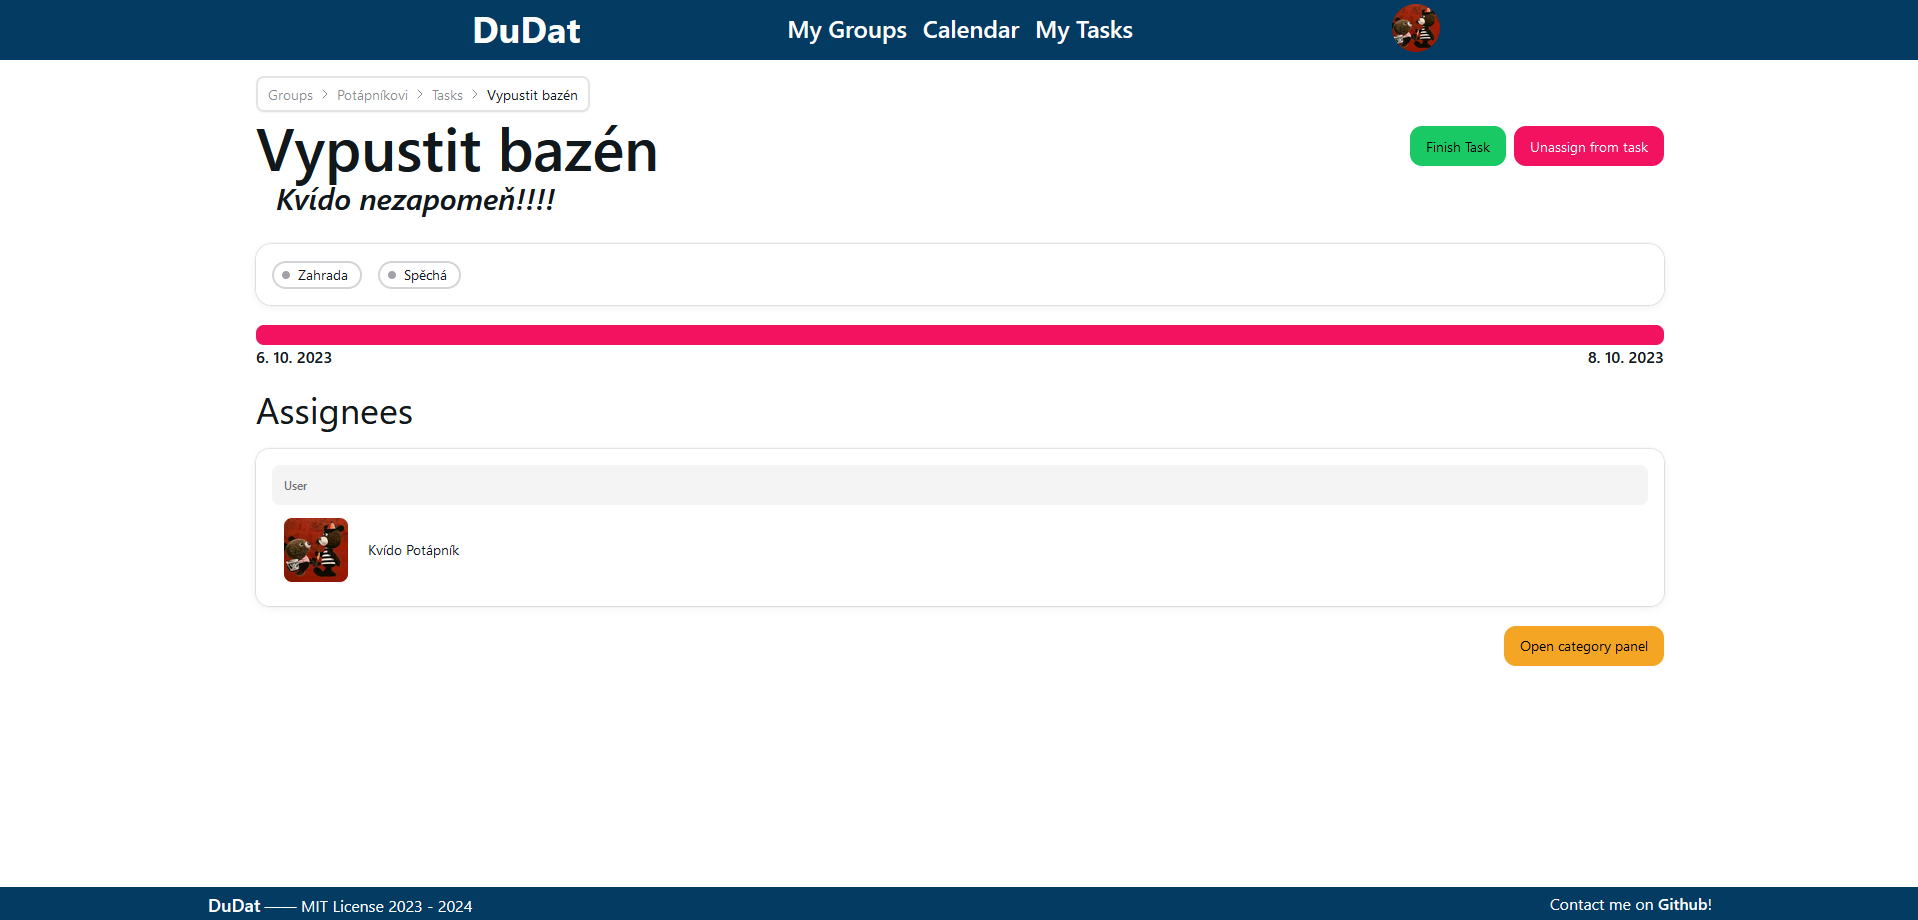
\includegraphics[width=1\linewidth]{img/opozdenyUkol.png}
	\caption{Zobrazení opožděného úkolu z pohledu uživatele}
\end{figure}

Po potvrzení autorem, nebo majitelem skupiny, že byl úkol vypracován, tak je indikátor vyšrafován. Pokud byl úkol dokončen v čas tak zezelená, jinak zůstane červený a nad indikátorem se zobrazí text, kdy byl úkol dokončen, ne kdy byl potvrzen jako dokončený.

\begin{figure}[hbt!]
	\centering
	
\includegraphics[width=1\linewidth]{img/progressOnTime.png}
	\caption{Zobrazení indikátoru u úkolu, který byl potvrzen a včas odevzdán}
\end{figure}

Dále se v aplikaci nachází i zobrazení kalendáře na stránce \code{tasks/calendar/}. Kalendář je řešen knihovnou \code{react-big-calendar}. Položky v kalendáři odkazují na svou stránku, dále se mění jejich zbarvení stejně jako v indikátoru na stránce úkolů.

\subsection{Úkoly x Přání}

Jako přání je v aplikaci brán jakýkoliv úkol, který nemá nikoho přiřazeného k sobě, zobrazují se tedy odděleně. Úkol je automaticky převeden na přání jakmile se odhlásí poslední člen od jeho plnění nebo pokud při vytváření nového úkolu zaškrtneme možnost, že se jedná o přání, v tom případě není po vytvoření automaticky přiřazen autor k plnění úkolu.

\begin{figure}[hbt!]
    \centering
    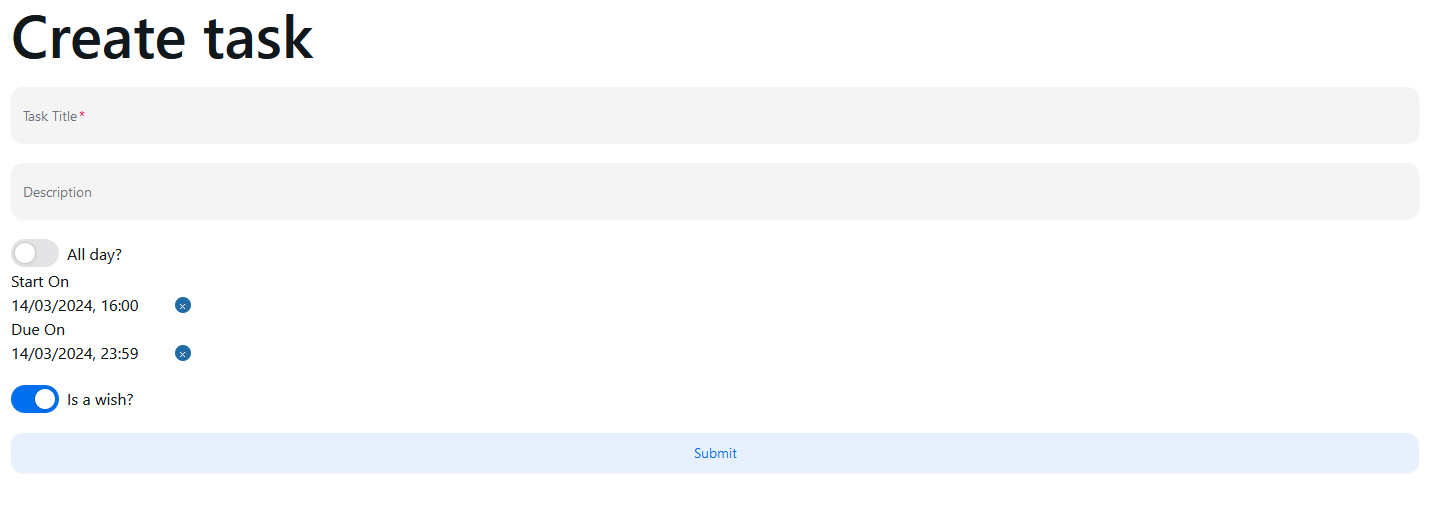
\includegraphics[width=1\linewidth]{img/taskCreate.png}
    \caption{Formulář pro vytvoření úkolu, který bude považován za přání}
\end{figure}
\newpage
Na stránce uživatele je kromě jejich jména a profilového obrázku zobrazeno grafové vyjádření, které porovnává počet úkolů, které splnil daný uživatel včas a počet úkolů, které odevzdal pozdě. Dále se zde nachází zobrazení takzvaného "Streak" systému, tedy jak dlouho to je, co uživatel odevzdal úkol pozdě. Pokud je uživatel na vlastní stránce tak se zde nachází tlačítko pro odhlášení a vstup na nastavení. V nastavení si může uživatel smazat svůj účet a změnit jméno.

\begin{figure}[hbt!]
	\centering
	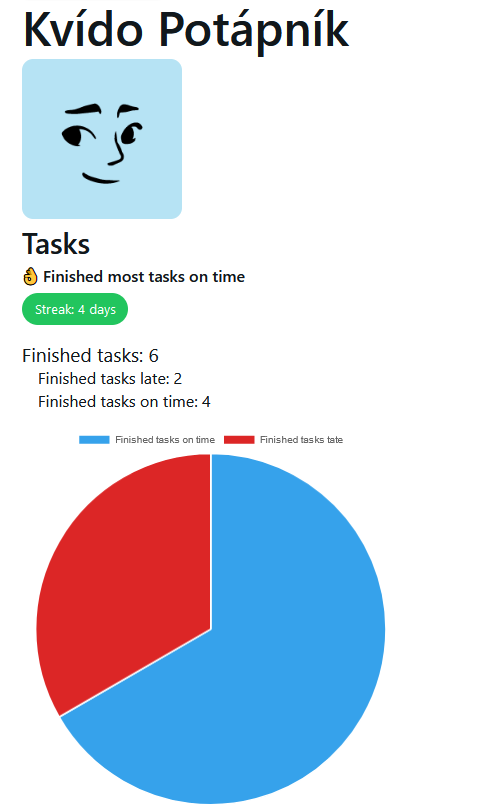
\includegraphics[height=0.5\textheight]{img/userPage.png}
	\caption{Zobrazení uživatelské stránky}
\end{figure}

Než bude uživateli dovoleno smazat svůj účet je potřeba, aby převedl veškeré skupiny, které vlastní na jiného uživatele nebo, aby skupinu smazal. Skupinu majitel převede na jiného uživatele v nastavení skupiny. Jakmile si uživatel smaže účet jsou všechny úkoly a kategorie, které vytvořil převedeny na majitele mateřské skupiny.